% --- Template for thesis / report with tktltiki2 class ---

\documentclass[finnish]{tktltiki2}

% tktltiki2 automatically loads babel, so you can simply
% give the language parameter (e.g. finnish, swedish, english, british) as
% a parameter for the class: \documentclass[finnish]{tktltiki2}.
% The information on title and abstract is generated automatically depending on
% the language, see below if you need to change any of these manually.
% 
% Class options:
% - grading                 -- Print labels for grading information on the front page.
% - disablelastpagecounter  -- Disables the automatic generation of page number information
%                              in the abstract. See also \numberofpagesinformation{} command below.
%
% The class also respects the following options of article class:
%   10pt, 11pt, 12pt, final, draft, oneside, twoside,
%   openright, openany, onecolumn, twocolumn, leqno, fleqn
%
% The default font size is 11pt. The paper size used is A4, other sizes are not supported.
%
% rubber: module pdftex

% --- General packages ---

\usepackage[utf8]{inputenc}
\usepackage{lmodern}
\usepackage{microtype}
\usepackage{amsfonts,amsmath,amssymb,amsthm,booktabs,color,enumitem,graphicx}
\usepackage[pdftex,hidelinks]{hyperref}

% Automatically set the PDF metadata fields
\makeatletter
\AtBeginDocument{\hypersetup{pdftitle = {\@title}, pdfauthor = {\@author}}}
\makeatother

% --- Language-related settings ---
%
% these should be modified according to your language

% babelbib for non-english bibliography using bibtex
\usepackage[fixlanguage]{babelbib}
\selectbiblanguage{finnish}

% add bibliography to the table of contents
\usepackage[nottoc,numbib]{tocbibind}
% tocbibind renames the bibliography, use the following to change it back
\settocbibname{Lähteet}

% --- Theorem environment definitions ---

\newtheorem{lau}{Lause}
\newtheorem{lem}[lau]{Lemma}
\newtheorem{kor}[lau]{Korollaari}

\theoremstyle{definition}
\newtheorem{maar}[lau]{Määritelmä}
\newtheorem{ong}{Ongelma}
\newtheorem{alg}[lau]{Algoritmi}
\newtheorem{esim}[lau]{Esimerkki}

\theoremstyle{remark}
\newtheorem*{huom}{Huomautus}


% --- tktltiki2 options ---
%
% The following commands define the information used to generate title and
% abstract pages. The following entries should be always specified:

\title{Iteratiiviset menetelmät}
\author{Jarl-Erik Malmström}
\date{\today}
\level{Aine}
\abstract{Tiivistelmä.}

% The following can be used to specify keywords and classification of the paper:

\keywords{agile, ketterä, open source, avoin}
\classification{} % classification according to ACM Computing Classification System (http://www.acm.org/about/class/)
                  % This is probably mostly relevant for computer scientists

% If the automatic page number counting is not working as desired in your case,
% uncomment the following to manually set the number of pages displayed in the abstract page:
%
% \numberofpagesinformation{16 sivua + 10 sivua liitteissä}
%
% If you are not a computer scientist, you will want to uncomment the following by hand and specify
% your department, faculty and subject by hand:
%
% \faculty{Matemaattis-luonnontieteellinen}
% \department{Tietojenkäsittelytieteen laitos}
% \subject{Tietojenkäsittelytiede}
%
% If you are not from the University of Helsinki, then you will most likely want to set these also:
%
% \university{Helsingin Yliopisto}
% \universitylong{HELSINGIN YLIOPISTO --- HELSINGFORS UNIVERSITET --- UNIVERSITY OF HELSINKI} % displayed on the top of the abstract page
% \city{Helsinki}
%


\begin{document}

% --- Front matter ---

\maketitle        % title page
\makeabstract     % abstract page

\tableofcontents  % table of contents
\newpage          % clear page after the table of contents


% --- Main matter ---

\section{Johdanto}

Tämän kirjoitelman tarkoituksena on tarkastella ohjelmistotuotannon iteratiivisia menetelmiä. Erilaisten ohjelmistotuotantomenetelmien historiaa, lähestymistapaa ohjelmistotuotantoon ja menetelmien heikkouksia sekä vahvuuksia. 

Kirjoitelma käy lyhyesti läpi erilaisia lähestymistapoja ohjelmistotuotantoon. Lisäksi tarkastellaan ohjelmistotuotantoprojektien erityispiirteitä ja ohjelmistotuotannon riskien tunnistamista, sekä miten nämä vaikuttavat menetelmän valintaan. 

Vaikka monet pitävät iteratiivisia ohjelmistotuotantomenetelmiä nykyaikaisina menetelminä, on niitä sovellettu ohjelmistokehityksessä 1950-luvulta lähtien. Winston Roycen ajatukset artikkelissa “Managing the Development of Large Software Systems,” loivat perustan vesiputousmallille, joka vastasi valtionhallinnon sopimusten rajoitteisiin. Monet pitävät virheellisesti Roycen artikkelia lineaarisen vesiputousmallin esikuvana. Roycen artikkelin iteratiivinen ja palautteenohjaama ohjelmistokehitys, jossa onjelmisto toteutetaan kahdesti, on unohtunut useista menetelmän kuvauksista.\cite{LAB03}

Ohjelmistotuotannossa on kaksi perustavanlaatuista vaihetta: analysointivaihe ja rakennusvaihe. Nämä kaksi vaihetta riittävät ohjelmiston totetuttamiseen, jos ohjelmisto on pieni ja tuotettavan ohjelmiston käyttäjät ovat itse toteuttajia.\cite{ROY70} 

Tällaisesta ohjelmistokehityksestä myös asiakkaat ovat valmiita maksamaan, sillä vaiheet pitävät sisällään aidosti luovaa työtä, joka suoraan edistää tuotettavan ohjelmiston käytettävyyttä.\cite{ROY70}

Suuremman ohjelmistotuotantoprojektin täytäntöönpano vaatii lisäksi muita vaiheita, jotka eivät suoraan edistä tuotettavaa ohjelmistoa ja lisäksi kasvattavat ohjelmistotuotannon kustannuksia.\cite{ROY70}

Ohjelmistotuotannon alkuaikoina käytetty ''ohjelmoi ja korjaa'' -mallin sisältää kaksi vaihetta. Ohjelmoidaan ensin ja mietitään vaatimuksia, rakennetta sekä testausta myöhemmin. Mallilla oli useita heikkouksia. Usean korjausvaiheen jälkeen ohjelmakoodi oli niin vaikeasti rakennettu, että oli hyvin kallista muuttaa koodia. Tämä korosti tarvetta suunnitteluvaiheelle ennen ohjelmointia.\cite{BOE88}

Usein hyvin suunniteltu ohjelmisto ei vastannut käyttäjien toiveita. Joten syntyi tarve vaatimusmäärittelylle ennen suunnitteluvaihetta.\cite{BOE88} 

Ohjelmistot olivat usein kalliita korjata koska muutoksiin ja testaamiseen oli valmistauduttu huonosti. Tämä osoitti tarpeen eri vaiheiden tunnistamiselle, sekä tarpeen huomioida testaus ja ohjelmiston muuttuminen jo hyvin varhaisessa vaiheessa.\cite{BOE88} 

   

\section{Ohjelmistotuotantomenetelmät}

\subsection{Vesiputousmalli}

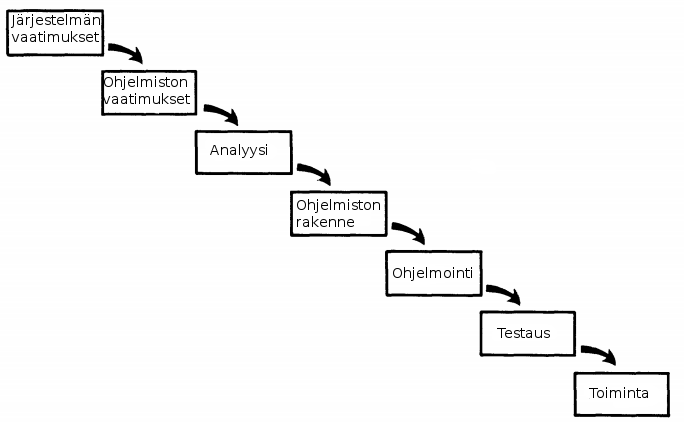
\includegraphics[width=\textwidth]{waterfall}

\subsubsection{Vaiheet}
1970-luvulla vesiputousmalli vaikutti suuresti lineaarisiin ohjelmistotuotannon malleihin. Vesiputousmallin lähestymistapa auttoi poistamaan monia aiemmin ohjelmistotuotantoa vaivanneita ongelmia. Vesiputousmallista tuli perusta monille teollisuuden ja hallituksen ohjelmistohankintojen standardeille. \cite{BOE88}

Tarkemmin Winston W. Roycen malli sisältää seuraavat vaiheet: järjestelmä- ja ohjelmistovaatimusmäärittely, analyysi, ohjelmistonrakenteen suunnittelu, ohjelmointi, testaus ja ohjelmiston käyttäminen.\cite{ROY70} 

Perättäisten ohjelmistotuotantovaiheiden välillä on iteraatiota järjestelmän rakenteen tarkentuessa yksityiskohtaisemmaksi tuotannon edetessä. Iteraatioiden tarkoituksena on suunnitelman edetessä pitää muutosvauhti käsiteltävän kokoisena.\cite{ROY70}

\subsubsection{Ohjelmiston suunnittelu}

Lineearinen ohjelmistotuotantoprosessi sisältää huomattavan riskin. Vasta testivaiheessa, menetelmän loppupuolella, saattaa tulla esille ilmiöitä, joita ei ollut mahdollista tarkalleen analysoida aikaisemmassa vaiheessa.\cite{ROY70}

Ellei pieni muutos koodissa korjaa ohjelmistoa vastaamaan oletettua käytöstä, vaadittavat muutokset ohjelmiston rakenteeseen saattavat olla niin häiritseviä, että muutokset rikkovat ohjelmistolle asetettuja vaatimuksia. Tällöin joko vaatimuksia tai suunnitelmaa on muutettava. Tässä tapauksessa tuotantoprosessi on palannut alkuun ja kustannusten voidaan olettaa nousevan jopa 100\%.\cite{ROY70}

Ongelman korjaamiseksi vaatimusmäärittelyn jälkeen - ennen analyysia - on tehtävä alustava rakenteen suunnittelu. Näin ohjelmistosuunnittelija välttää talletamiseen tai aika -ja tilavaatimuuksiin liittyvät virheet. Analyysin edetessä ohjelmistosuunnittelijan on välitettävä aika- ja tilavaatimukset sekä operatiivisiset rajoitteet analyysin tekijälle.\cite{ROY70}

Näin voidaan tunnistaa projektille varatut alimitoitetut kokonaisresurssit tai virheelliset operatiiviset vaatimukset aikaisessa vaiheessa. Vaatimukset ja alustava suunnitelma voidaan iteroida ennen lopullista suunnitelmaa, ohjelmointia ja testausvaihetta.\cite{ROY70}

\subsubsection{Dokumentointi}

On laadittava ymmärrettävä, valaiseva ja ajantasainen dokumentti, jonka jokaisen työntekijän on sisäistettävä.\cite{ROY70}

Vähintään yhden työntekijällä on oltava syvällinen ymmärrys koko järjestelmästä, mikä on osaltaan saavutettavissa dokumentin laadinnalla.\cite{ROY70}

Ohjelmistuotannon hyvin tärkeä sääntö on erittäin kattava dokumentointi. Ohjelmistosuunnittelijoiden on kommunikoitava rajapintojen(interface) suunnittelijoiden, ja johdon kanssa. Dokumentti antaa ymmärrettävän perustan rajapintojen suunnitteluun ja hallinnollisiin ratkaisuihin.\cite{ROY70}

Kirjallinen kuvaus pakottaa ohjelmistosuunnittelijan yksiselitteiseen ratkaisuun ja tarjoaa konkreettisen todistuksen työn valmistumisesta.\cite{ROY70}

Hyvän dokumentoinnin todellinen arvo ilmenee tuotannossa myöhemmin testausvaiheessa, ohjelmistoa käytettäessä sekä uudelleen suunniteltaessa.\cite{ROY70}

Hyvän dokumentin avulla esimies voi keskittää henkilöstön ohjelmistossa ilmenneisiin virheisiin. Ilman hyvää dokumenttia, ainoastaan ohjelmistovirheen alkuperäinen tekijä kykenee analysoimaan kyseessä olevan virheen.\cite{ROY70}

Dokumentti helpottaa ohjelmiston käyttöönottoa operatiivinen henkilöstön kanssa. Käyttöönotossa ilmenneiden mahdollisten ohjelmistovirheiden korjaamisessa selkeä dokumentti on välttämätön.\cite{ROY70}   

\subsubsection{Toinen versio}

Dokumentoinnin jälkeen toinen ohjelmistoprojektin onnistumiseen vaikuttava tärkein tekijä on sen alkuperäisyys. Jos kyseessä olevaa ohjelmistoa kehitetään ensimmäistä kertaa, on asiakkaalle toimitettava käyttöönotettava versio oltava toinen versio, mikäli kriittiset rakenteelliset ja operatiiviset vaatimukset on huomioitu.\cite{ROY70} 

Lyhyessä ajassa suhteessa varsinaiseen aikatauluun suunnitellaan ja rakennetaan prototyyppiversio ennen varsinaista rakennettavaa ohjelmistoa. Jos suunniteltu aikataulu on 30 kuukautta, niin pilottiversion aikataulu on esimerkiksi 10 kuukautta. Ensimmäinen versio tarjoaa aikaisen vaiheen simulaation varsinaisesta tuotteesta.\cite{ROY70}

\subsubsection{Testaus}

Testaus on projektin resursseja vaativin vaihe. Testausvaiheessa vallitsee suurin riski taloudellisesti ja ajallisesti. Loppuvaiheessa aikataulua on vähän varasuunnitelmia tai vaihtoehtoja. Alustava suunnitelma ennen analysointia ja ohjelmointia sekä prototyypin valmistaminen ovat ratkaisuja ongelmien löytämiseen ja ratkaisemiseen ennen varsinaiseen testivaiheeseen siirtymistä.\cite{ROY70}

Testivaiheen tulee pääasiallisesti suorittaa siihen erikoistunut asiantuntija, joka ei välttämättä osallistunut varsinaiseen ohjelmointiin. Väite, että ohjelmistosuunnittelija on paras henkilö      
testaamaan suunnitelemansa ohjelmiston, koska ymmärtää aihealueen parhaiten, on merkki siitä että dokumentointi ei ole ollut riittävää.\cite{ROY70} 

Useimmat virheet ovat luonteeltaan ilmiselviä, jotka voidaan löytää visuaalisella tarkastelulla. Jokaisen analyysin ja ohjelmakoodin tulee tarkastaa toinen henkilö, joka ei osallistunut varsinaiseen työhön. Jokainen tietokoneohjelman looginen polku on testattava ainakin kerran.\cite{ROY70}
 
\subsubsection{Asiakas}

Jostain syystä ohjelmiston suunnitelmaan ja aiottuun toimintaan sovelletaan laajaa tulkintaa, jopa aikasemman yhteisymmärryksen jälkeen. On tärkeää sitouttaa asiakas formaalilla tavalla mahdollisimman aikaisessa vaiheessa projektia, näin asiakkaan näkemys, harkinta ja sitoumus vahvistaa kehitystyötä.\cite{ROY70} 	  


\subsection{Iteratiiviset menetelmät}

\subsubsection{Vesiputousmallin heikkous}
Lineaarisesti vaiheesta toiseen etenevän ohjelmistotuotantomentelmä ei sovi erityisesti interaktiivisiin loppukäyttäjien sovelluksiin. Suunnitelmaperustaiset standardit pakottavat dokumentoimaan yksityiskohtaisesti heikosti ymmärretyt käyttöliittymien vaatimukset.\cite{BOE88}

Tästä seurasi käyttökelvottoman ohjelmakoodin suunnittelua ja toteutusta. Lineaarisen ohjelmistotuotantomenetelmän vaiheet olivat tällaisille projekteille selvästi väärässä järjestyksessä. Erityisesti joillekin ohjelmistoille ei ole tarvetta yksityiskohtaiselle dokumentaatiolle ennen toteutusta.\cite{BOE88}

\subsubsection{Iteratiivinen ja inkrementaalinen}

NASA:n käytti iteratiivista ja inkrementaalista (IID) ohjelmistotuotantomentelmää Mercury-projektissa 1960-luvulla. Mercury-projekti toteutettiin puolen päivän iteraatioissa. Kehitystiimi sovelsi Extreme programming-menetelmän käytänteitä tekemällä testit ennen jokaista pientä inkremen\-taatiota.\cite{LAB03}

IBM:n FSD (Federal System Division) yksikkö käytti 1970-luvulla laajasti ja onnistuneesti iteratiivisia ja inkrementaalisia menetelmiä kriittisissä Yhdysvaltain puolustusministeriön avaruus- ja ilmailujärjestelmien kehityksessä.\cite{LAB03}

Vuonna 1972 miljoonan koodirivin Trident-sukellusveneen komento- ja ohjausjärjestelmän kehityksessä osasto organisoi projektin neljään noin kuuden kuukauden iteraatioon. Projektissa oli merkittävä suunnittelu- ja määrittelyvaihe sekä iteraatiot olivat nykyisen ketterän kehityksen (agile methods) suosituksia pidempiä. Vaatimus\-määrittely kuitenkin kehittyi palautteen ohjaamana. Iteratiivisella ja inkrementaalisella lähestymistavalla hallittiin monimutkaisuutta sekä riskejä suuren mittakaavan ohjelmistoprojektissa. Toimittajaa uhkasi myöhästymisestä 100 000\$ uhkasakko per päivä.\cite{LAB03}

IBM:n FSD osasto kehitti Yhdysvaltain laivastolle suuren mittaluokan asejärjestelmän iteratiivisella ja inkrementaalisella mentelmällä. neljän vuoden, 200 henkilötyövuoden ja miljoonien ohjelmarivien projekti toteutettiin 45:ssä yhden kuukauden mittaisissa aikarajoitetuissa (time-boxed) iteraatiossa. Tämä oli ensimmäisiä ohjelmistoprojekteja, joka käytti nykyisten ketterien menetelmien suosittelemia iteraatiojakson pituutta.\cite{LAB03}

\subsubsection{Spiraalimalli}

Spriraalimalli on kehitetty vesiputousmallista saatujen  useiden vuosien kokemuksien perusteella. Malli kuvastaa taustalla olevaa käsitettä, että jokainen vaihe sisältää saman sarjan toimenpiteitä.\cite{BOE88}

Jokainen vaihe aloitetaan tunnistamalla:
\begin{itemize}
  \item laadittavien ohjelmisto-osien suorituskykyyn, toiminnallisuuteen sekä sopeutumiskykyyn liittyvät tavoitteet
  \item vaihtoehtoiset toteutustavat (ohjelmiston osto, ohjelmiston uudelleenkäyttö, vaihtoehtoiset ohjelmat)
  \item ohjelmiston eri vaihtoehdoille asettamien rajoitteet (rajapinnat, aikataulu, kustannukset).
\end{itemize}\cite{BOE88}

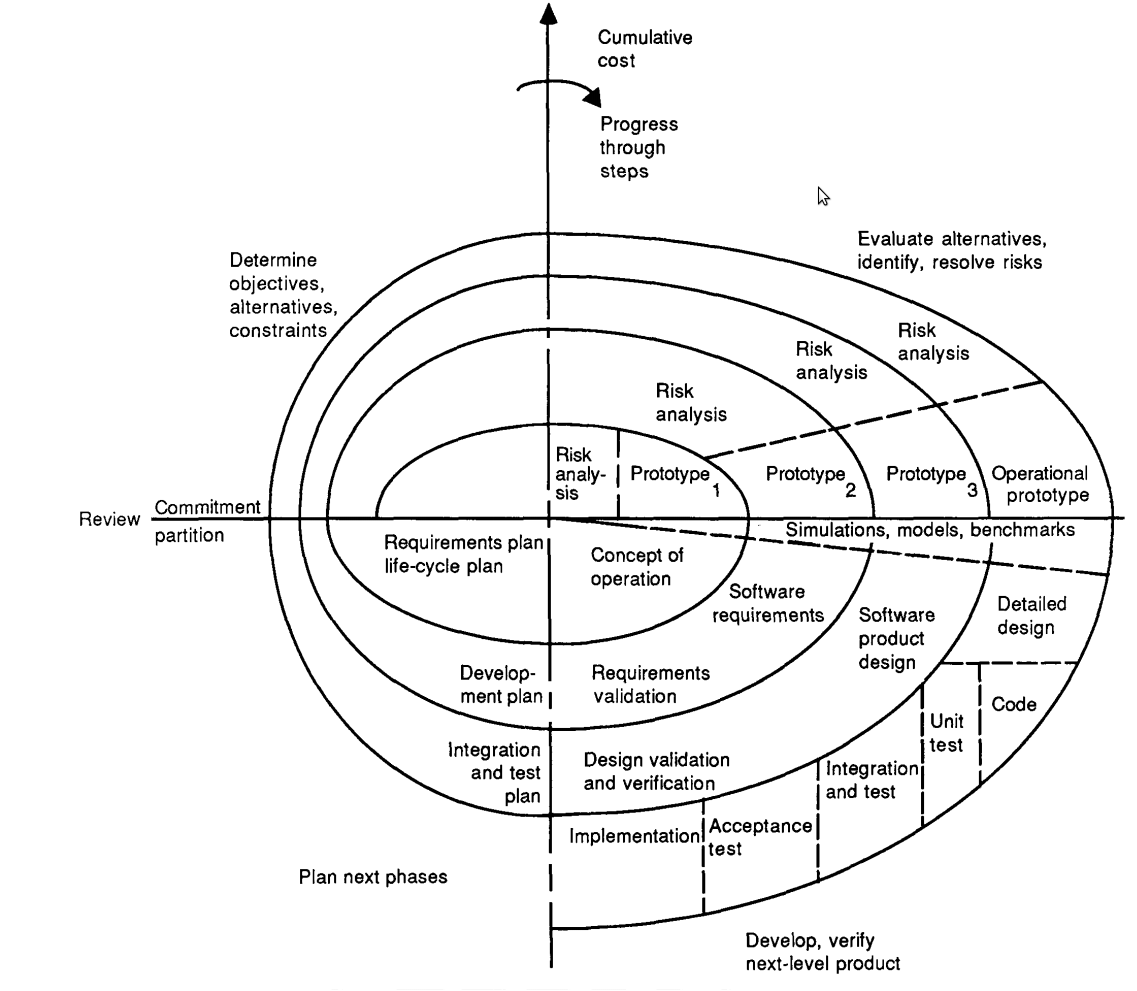
\includegraphics[width=\textwidth]{spiral}

Seuraava askel on arvioida vaihtoehtoja suhteessa ohjelmiston tavoitteisiin ja rajoitteisiin. Usein tämä prosessi tunnistaa epävarmoja alueita, jotka ovat merkittäviä riskin lähteitä. Riskien löytyessä, seuraava askel pitää sisällään kustannustehokkaan strategian muotoilun riskien ratkaisemiseksi. Tähän voi liittyä prototyyppien valmistamista, simulointia, vertailuanalyysia, kyselylomakkeita, analyyttista mallinnusta, tai näiden yhdistelmiä sekä muita riskien ratkaisumenetelmiä.\cite{BOE88}


Jos suorituskykyyn tai käyttöliittymään liittyvät riskit voimakkaasti hallitsevat ohjelman kehittämistä, seuraavassa vaiheessa kehityksellisesti (evolutionary), mahdollisimman vaivattomasti, määritellään ohjelmiston yleistä luonnetta, suunnitellaan seuraavan tason prototyyppia ja kehitetään yksityiskohtaisempaa prototyyppia riskien ratkaisemiseksi.\cite{BOE88}

Spriraalimalli on jaoteltu vaiheisiin riskiperusteisesti. Tämä mahdollistaa mallin mukautumaan sopivasti yhdistelemällä erittelyä (specification), prototyyppien valmistusta, simulointia tai muita lähestymistapoja ohjelmiston suunnitteluun.\cite{BOE88}

Riskinhallinta huomioiden voidaan määritellä kiinnitettävä aika ja työmäärä toiminnan suunnitteluun (planning), asetuksien hallintaan (configuration management), laadun varmistukseen(quality assurance), muodolliseen todentamiseen (formal verification) ja testaukseen.\cite{BOE88}

Spiraalimallin tärkeä ominaisuus on, että jokainen iteraatio päätetään katselmukseen tuotteeseen liittyvän henkilöstön tai organisaation kanssa.\cite{BOE88}

\subsection{Ketterät kehitysmenetelmät}

\section{Ohjelmistojen laadun varmistus}

\subsection{Ohjelmistotuotannon ominaispiirteet}

Onnistunut ohjelmistojärjestelmä vaatii erilaisten pyrkimysten koordinointia ohjelmistokehityksen aikana. Ohjelmistojärjestelmien perustavanlaatuinen ominaisuus on niiden suuri koko. Yksilöiden tai pienten ryhmien on mahdotonta luoda tai ymmärtää suuria ohjelmistoja yksityiskohtaisesti.\cite{KES95}

Suuret projektit onnistuvat useimmin jos projektia koordinoi henkilö, jolla on tietoa ohjelmiston toimialalta sekä ohjelmistolalta.\cite{KES95}

Tällainen ideaalitilanne on usein mahdotonta suurille ohjelmistojärjestelmille, jonka koko voi olla miljoonia tai kymmeniä miljoonia ohjelmarivejä sekä projektin kesto useita vuosia.\cite{KES95}

Suuren kokoluokan pyrkimykset johtavat erikoistumiseen ja työn jakamiseen. Organisaatiossa tämä johtaa toisistaan riippuvien tekijöiden jakamiseen osastoihin maantieteellisesti, organisatorisesti, sekä sosiaalisesti. Tämä vähentää mahdollisuuksia ja haluja oppia sekä jakaa tietoa etäisten työtovereiden kesken.\cite{KES95}

\subsubsection{Epävarmuus}
Luontainen epävarmuus lisää koordinointiongelmaa. Toisin kuin teollinen valmistus, ohjelmistokehitys ei ole rutiininomainen toimi. Monet ohjelmistojärjestelmät ovat yksilöllisiä projekteja, ilman olemassa olevaa prototyyppiä, tai muokattavaa ohjelmistoa.\cite{KES95}


Lisäksi epävarmuus lisääntyy, koska ohjelmiston toimintaan liittyvät vaatimukset muuttuvat. 

Muutoksia ohjelmiston vaatimuksiin esiintyy, koska ympäristö mihin ohjelmisto suunniteltiin muuttuu. Liiketoiminta, käyttäjien toiveet, tietokoneympäristö, ohjelmiston syötteet ja fyysinen maailma itsessään muuttuvat. 

Muutostarpeiden ilmaantumisen todennäköisyys on suurin ohjelmistoa käytettäessä. Tällöin käyttäjät usein ymmärtävät ohjelmiston rajoitteet ja mahdollisuudet. Kun ohjelmistoa käytetään olosuhteissa, johon sitä ei ollut alunperin kuviteltu alkuperäistä suunnitelmaa tehtäessä, niin käyttäjät todennäköisesti vaativat uusia toiminnallisuuksia. \cite{KES95}

Ohjelmistokehitys on epävarmaa, koska vaatimukset ovat poikkeuksetta epätäydellisiä. Epätäydellisyys aiheutuu osittain rajallisista toimialan tiedoista ja ohjelmistoprojektin tyypillisestä työn jakamisesta. Liian vähällä, projektissa työskentelevillä ihmisillä, on riittävää tuntemusta toimialasta. \cite{KES95}

Tyypillisesti analyytikko vaihtelevalla toimialan tuntemuksella haastattelee asiakkaita ja käyttäjiä. Tämän jälkeen analyytikko kirjoittaa vaatimukset ohjelmistoarkkitehdeille ja -suunnittelijoille. Tässä prosessissa merkityksellistä toimialatietoa poikkeuksetta katoaa.\cite{KES95}

Kaikkia käyttäjien tarpeita analyytikko ei löydä ja jotkin tarpeet jäävät kirjaamatta vaatimusmäärittelyyn. Suuri koordinointiongelma ohjelmistokehityksessä on, että ohjelmistoarkkitehtien ja -suunnittelijoiden päätöksentekoon tarvitsema tieto ei ole saatavilla käytettävissä olevissa dokumenteissa.\cite{KES95}

\subsubsection{Keskinäiset riipuvuudet}
Suuri kokoluokka ja epävarmuus olisivat vähäisempiä ongelmia, jos ohjelmisto ei vaatisi sen osajärjestelmien täsmällistä integraatiota. Ohjelmistot pääasiallisesti ovat rakennettu useista osista, jotka on kytkettävä yhteen, jotta ohjelmisto toimisi oikein.\cite{KES95}

\subsubsection{Epävirallinen keskustelu}
Käytännön kokemus ja organisaatio teoria osoittavat, että aikaisemmat ohjelmistotuotannon aikaansaannokset eivät ole onnistuneet ratkaisemaan suurien ohjelmistoprojektien kooridinointiongelmia. 
Voidaan sanoa, että aikaisemmat ehdotetut korjaustoimenpiteet ovat lähestyneet ongelmaa seuraavasti: 
\begin{itemize}
 \item Tekniset työkalut, kuten tekstimuokkain (editor) tai korkean tason kielet
 \item Ohjelmiston jakaminen osiin (modularization) teknisesti, esimerkiksi olio-ohjelmoinnilla (object-oriented programming). Tai hallinnollisesti vaatimusmäärittelyn, ohjelmoinnin ja testaus toimintojen eriyttämisellä.
 \item Teknisillä formaaleilla menettelytavoilla,esimerkiksi versionhallinta, testisuunnitelma ja vaatimusmäärittelydokumentit.
\end{itemize}
\subsubsection{Kymmenen ohjelmistotuotannon riskiä}

\begin{enumerate}
  \item Henkilöstö vaje.
  \item Epärealistinen aikataulu ja budjetti.
  \item Väärien ohjelmiston toiminnallisuuksien kehitys.
  \item Vääränlaisen käyttöliittymän kehitys.
  \item Ohjelmiston ominaisuuksien parantelu vaatimusten täytyttyä.
  \item Jatkuvasti vaihtuvat vaatimukset.
  \item Puutteet ulkoisesti toimitetuissa ohjelmiston osissa.
  \item Puutteet ulkoisesti suoritetuissa tehtävissä.
  \item Puutteet reaaliaikaisuuden suorituskyvyssä.
  \item Tietojenkäsittelytieteen valmiuksien ylikuormitus.
\end{enumerate}\cite{BOE88}

\section{Ohjelmistotuotantomenetelmän valinta}

\subsection{Ennustettavuus}

\subsection{Muuttuva liiketoimintaympäristö}

\subsection{Organisaation koko}

\subsection{Kehittäjien taidot}

\subsection{}

\section{}

\section{}


% --- Back matter ---
%
% bibtex is used to generate the bibliography. The babplain style
% will generate numeric references (e.g. [1]) appropriate for theoretical
% computer science. If you need alphanumeric references (e.g [Tur90]), use
%
% \bibliographystyle{babalpha}
%
% instead.

\bibliographystyle{babplain}
\bibliography{references-fi}


\end{document}
